\documentclass[11pt]{article}
\usepackage[margin=1in]{geometry}
\usepackage{times}
\usepackage{amsmath,amssymb}
\usepackage{booktabs}
\usepackage{graphicx}
\usepackage{xcolor}
\usepackage{url}
\usepackage[colorlinks=true,linkcolor=blue!60!black,citecolor=blue!60!black,urlcolor=blue!60!black]{hyperref}
\usepackage[round,authoryear]{natbib}
\usepackage{caption}
\captionsetup{font=small,labelfont=bf}
\setlength{\parskip}{0.35em}

\title{\textbf{TabICL-M: A Tabular Foundation Model that Reads Missingness as Provenance}}
\author{Sompote Youwai\\
King Mongkut's University of Technology Thonburi, Bangkok, Thailand\\
\texttt{sompote.you@kmutt.ac.th}\\[0.4em]
\small Code, weights and every result table: \url{https://github.com/Sompote/TabICL-M}}
\date{September 2026}

\begin{document}
\maketitle

\begin{abstract}
Engineering databases are rarely measured by one instrument. They are merged from
laboratories, sites and campaigns, each of which recorded its own subset of the
features with its own calibration, so the resulting table has block-structured
gaps and per-source offsets rather than random holes. Tabular foundation models
handle missing values cell by cell, either by imputation or by a missingness
indicator, and we show that on such data this is where they all lose: when the test
rows come from a source the context has never seen, TabICLv2, TabPFN~2.5, TabPFN-3,
classical imputers and gradient-boosted trees give up 0.02--0.08 AUC or 1--3 RMSE
beyond what the gaps themselves cost, and none recovers it. We present TabICL-M, a
continuation of TabICLv2 built on one observation: in a merged table, rows that share
a missingness pattern come from the same source, so the pattern is free, label-free
provenance. TabICL-M encodes each value relative to the statistics of its own
pattern group, represents each row from its observed features only, and carries a
pattern token into in-context learning; it is trained with a block-structured
missingness prior with per-source offsets, a block-reconstruction objective and an
offset-consistency loss. All additions are zero-initialised, so on complete data the
model equals TabICLv2 exactly. On 20 datasets with injected block missingness (5
seeds, held-out-source and random splits) TabICL-M is the best model of any kind
when a held-out source carries a measurement offset (mean rank 2.22 against 2.45 for
TabPFN-3; 14 of 20 datasets won), level with TabPFN-3 on classification, and behind it
only on plain regression, for reasons we trace to the base regressor rather than to
the method. It reaches this with half the parameters and a third of the inference
time of TabPFN-3. We report every negative result on the way, including that a
TabPFN-style histogram head, test-time fine-tuning and continued training do not
close the plain-regression gap.
\end{abstract}

\section{Introduction}

A foundation model for tabular data is pre-trained once on synthetic tables and then
applied to a new table by in-context learning: the labelled rows are the context, the
unlabelled rows are the queries, and no gradient step is taken \citep{hollmann2023tabpfn,
hollmann2025tabpfnv2, qu2025tabicl}. These models now lead the public leaderboards on
small and medium tables \citep{erickson2025tabarena}. They are trained, however, on
complete synthetic tables, and the missing values they meet in practice are treated
as a nuisance to be smoothed away, by imputation in the preprocessing or by a
cell-wise missingness indicator in the encoder \citep{hollmann2025tabpfnv2}.

The tables that motivate this work look different. A geotechnical compaction database,
the case that started the project, is a union of records from several laboratories;
each laboratory measured the properties it had equipment for, and the same physical
quantity measured in two laboratories differs by an offset. The result is a table in
which the missingness is \emph{block-structured} (a laboratory lacks whole columns, not
scattered cells) and \emph{informative about the source} (which columns a row lacks
tells you where it came from), and in which the features carry a per-source shift. A
model that imputes the column mean into a laboratory's unmeasured columns, and treats
the shifted values of another laboratory as if they were on a common scale, is biased
in a way that no amount of context can correct.

Before building anything we asked where the headroom is. We took complete public
tables, split their rows into synthetic sources, gave each source its own feature
subset and optionally its own offset, and evaluated the released TabICLv2 under two
splits: a random split, in which every source appears in the context, and a
leave-one-source-out split, in which the test rows come from a source the context has
never seen. The finding (Section~\ref{sec:headroom}) is sharp. Under the random split
the source offset costs nothing: in-context learning calibrates it away, and mean
imputation inside an in-context learner is already close to the information limit, so
that no method, including TabPFN~2.5 and TabPFN-3, is separable from any other. Under
the held-out source the same offset costs 0.02--0.08 AUC or 1--3 RMSE on every
dataset, on top of the loss from the gaps, and every existing method loses it:
imputers lose more than mean imputation, trees more still, and TabPFN as much as
TabICL. That loss is a nuisance offset on values that are all present, not lost
information, and it is the case a merged database presents every time a new source
arrives.

TabICL-M targets exactly that case. Its principle is that the missingness pattern of a
row is its provenance. Section~\ref{sec:method} turns this into three additions to the
three stages of TabICLv2 and two training objectives, all of which are
zero-initialised or identity on complete data so that the model starts, and on complete
tables stays, exactly at the released TabICLv2. Section~\ref{sec:training} describes the
continued pre-training on synthetic data only, Section~\ref{sec:experiments} the
benchmark against the released model, classical imputers, gradient-boosted trees and
four versions of TabPFN, the ablation of each part on both tasks, and the negative
results, and Section~\ref{sec:discussion} what the whole says about where the
remaining gap to TabPFN-3 lies.

\paragraph{Contributions.}
(i) A headroom study showing that the only regime in which current tabular foundation
models leave a recoverable gap on incomplete data is a held-out source with its own
feature subset and measurement offset. (ii) A source-aware architecture that reads a
row's missingness pattern as provenance, with a source-relative value encoding,
observed-only row attention and a pattern token, plus a block-structured prior and two
objectives that train it, all bit-exact to TabICLv2 on complete data. (iii) The first
tabular foundation model that beats TabPFN-3 when a new source carries an offset, at
half its size and a third of its inference time, while remaining level with it on
classification. (iv) A complete record of what did not work, so that the plain
regression gap is attributed correctly to the base regressor.

\section{Related work}

\paragraph{Tabular foundation models.} TabPFN \citep{hollmann2023tabpfn} introduced
in-context learning on synthetic tables drawn from structural causal models; TabPFN~v2
\citep{hollmann2025tabpfnv2} extended it to regression and larger tables, injected
cell-wise missingness into its prior and added a missing indicator to its encoder.
TabPFN~2.5 and TabPFN-3 are the current releases of that line; we compare against all
of them. TabICL \citep{qu2025tabicl} and TabICLv2 \citep{qu2026tabiclv2} factor the
model into a column-wise set transformer \citep{lee2019set}, a row-wise transformer
and a dataset-wise in-context learner, which scales to hundreds of thousands of rows.
TabICL-M is a fork of TabICLv2 and inherits that structure.

\paragraph{Missing values in deep tabular models.} NAIM \citep{caruso2024naim} masks
missing features out of attention instead of imputing them, an idea our observed-only
row attention shares, inside an in-context learner. ReMasker \citep{du2024remasker}
and VIME \citep{yoon2020vime} train tabular models with masked-cell reconstruction; our
reconstruction objective hides blocks of columns of a pseudo-source rather than random
cells. All three treat missingness as cell-wise and random; none exploits the pattern as
a source identifier. Classical imputation, multiple imputation by chained equations in
particular \citep{vanbuuren2011mice}, is the standard preprocessing; we show it is
worse than mean imputation in front of an in-context learner. The distinction between
missing completely at random, at random and not at random goes back to
\citet{rubin1976inference}; block-structured, source-informative missingness fits none
of the three.

\paragraph{Source shift.} Normalising per domain to remove a nuisance shift is an old
idea in vision \citep{li2016adabn}. Our source-relative value encoding is its tabular,
label-free analogue, with the twist that the domain is inferred from the missingness
pattern and the normalised value is added as an input rather than replacing the raw
one, so that real between-source signal is not thrown away.

\paragraph{Benchmarks.} TabArena \citep{erickson2025tabarena} is a living benchmark of
tabular models on curated i.i.d.\ datasets; BeyondArena \citep{beyondarena2026} adds
temporal and grouped splits. Their datasets are complete, so they cannot show the
effect we target; we report results on them separately in the repository.

\section{Where the headroom is}
\label{sec:headroom}

We start from six complete public tables (breast cancer, wine, diabetes, credit-g,
adult, Boston housing), delete cells under a stated mechanism at a stated rate, and
compare models that handle the gaps in different ways. The \emph{block} mechanism
assigns rows to two to five sources and removes a different subset of columns from
each; \emph{block\_shift} additionally gives every source an additive offset
$\mathcal N(0, 0.5\sigma_j)$ and extra noise on each numeric feature $j$, imitating
laboratories that measure differently. Two splits are used: a stratified random split,
and a leave-one-source-out split in which one whole synthetic source is the test set.
Five seeds, rates 0.3 and 0.5.

\begin{table}[t]
\centering\small
\caption{The released TabICLv2 (mean imputation) at 50\,\% missingness. Source shift
costs nothing under a random split and 0.02--0.08 AUC or 1--3 RMSE under a held-out
source. Mean over 5 seeds.}
\label{tab:headroom}
\begin{tabular}{lccccc}
\toprule
dataset & complete & block, random & block, held-out & \textbf{block\_shift, held-out} & shift-specific loss\\
\midrule
adult (AUC) & 0.912 & 0.865 & 0.847 & \textbf{0.800} & $-0.047$\\
credit-g (AUC) & 0.814 & 0.722 & 0.704 & \textbf{0.683} & $-0.021$\\
wine (AUC) & 1.000 & 0.996 & 0.990 & \textbf{0.914} & $-0.076$\\
Boston (RMSE) & 2.71 & 4.84 & 5.84 & \textbf{7.08} & $+1.24$\\
diabetes (RMSE) & 55.8 & 65.3 & 66.4 & \textbf{69.1} & $+2.7$\\
\bottomrule
\end{tabular}
\end{table}

Table~\ref{tab:headroom} gives the base model's numbers. Three facts follow. First,
under the random split the offset is harmless, because every source is represented in
the context and in-context learning absorbs a constant per-source shift on its own.
Second, under the held-out source the offset costs every dataset a further 0.02--0.08
AUC or 1--3 RMSE. That loss is recoverable in principle: the values are all present,
only their scale is unknown. Third, every alternative loses more. Iterative imputation
in front of the same model is worse than mean imputation on all six datasets under the
held-out source (adult 0.677, wine $-0.042$ AUC, Boston $+1.35$ RMSE); $k$-nearest
neighbour imputation is worse still; XGBoost and CatBoost drop to 0.79 and 0.78 AUC on
adult and 8.6 and 9.5 RMSE on Boston; and TabPFN~v2 (0.816), TabPFN~2.5 (0.822) and
TabPFN-3 (0.812) sit in the same band as TabICLv2 on adult. The first-generation
TabICL-M checkpoint, which adds only value-level parts (a missing indicator, an absence
vector and cell-wise reconstruction), moved these numbers by less than the seed
spread. A fixed pattern-conditional normalisation recovers part of the shift loss
(adult $+0.025$ AUC) but hurts when there is no offset (credit-g $-0.012$), which is
the argument for learning the encoding instead of hard-coding it.

\section{Method}
\label{sec:method}

\begin{figure}[t]
\centering
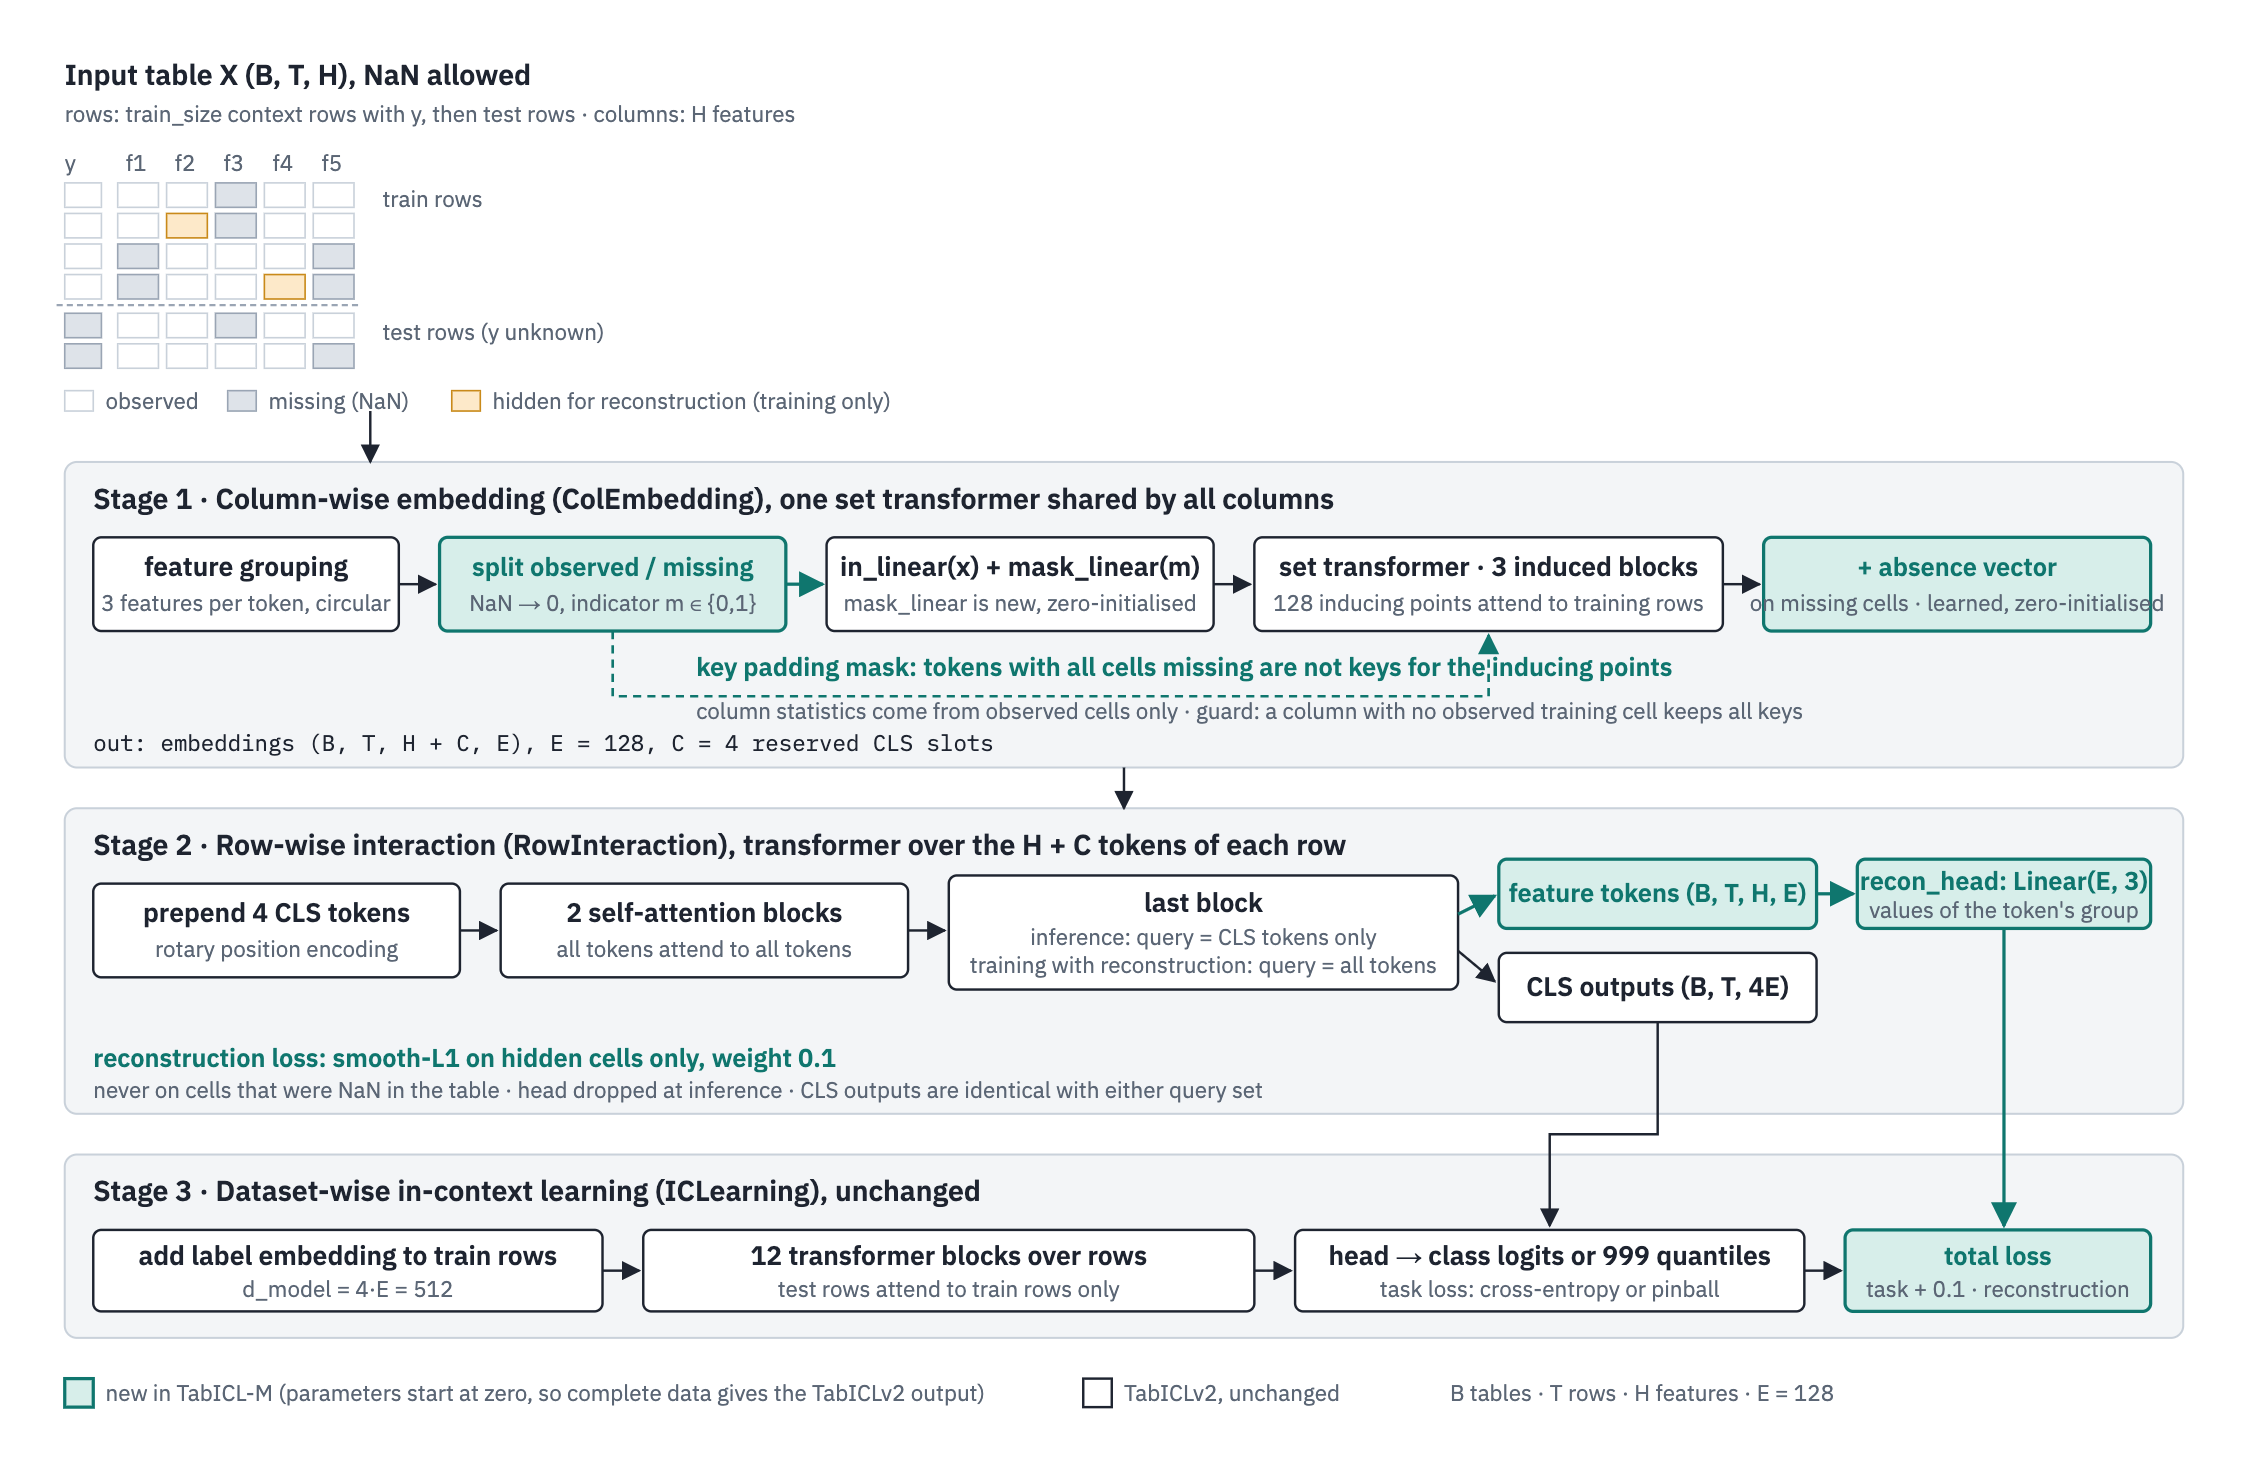
\includegraphics[width=\linewidth]{figures/architecture.png}
\caption{The three stages of TabICLv2 with the additions of TabICL-M in green. Every
new parameter starts at zero, so on a table with no missing cell the output is
identical to TabICLv2.}
\label{fig:arch}
\end{figure}

\subsection{The principle}

In a table merged from several sources, two rows that lack exactly the same columns
almost always come from the same source. The binary missingness pattern of a row is
therefore a source identifier that costs nothing, needs no provenance column and
survives any preprocessing that keeps NaN. TabICL-M uses it at every stage
(Figure~\ref{fig:arch}). We write a table as $X \in \mathbb R^{T\times H}$ with $T$
rows, $H$ features and NaN at missing cells, $m_{tj} = \mathbb 1[X_{tj}\ \text{missing}]$,
and $p(t) = (m_{t1},\dots,m_{tH})$ for the pattern of row $t$; the first $n$ rows carry
a label.

\subsection{Stage 1: source-relative value encoding}

TabICLv2 embeds each column with a set transformer whose 128 inducing points attend to
the labelled rows, so the column statistics that scale a value come from the whole
context. TabICL-M groups rows by pattern, $G(t) = \{t' : p(t') = p(t)\}$, and feeds every
observed cell twice: as its raw value and as
\begin{equation}
\tilde x_{tj} = \frac{x_{tj} - \mu_j(G(t))}{\sigma_j(G(t))},
\end{equation}
the value standardised within the rows of its own pattern group (patterns with fewer
than eight rows fall back to the table-wide statistics). Labelled and unlabelled rows
are pooled for these statistics, and no label is used, so a source that appears only
in the test rows is centred on itself. The two values enter the token through separate
linear maps, $\mathrm{in}(x) + \mathrm{rel}(\tilde x) + \mathrm{mask}(m)$, and the
map $\mathrm{rel}$ is zero-initialised. Because the raw value is still present, the
model can learn how much of a between-source difference is nuisance and how much is
signal, instead of having that decided by a fixed normalisation. Missing cells are
zero-filled, hidden from the keys of the inducing-point attention so that statistics
come from observed cells only, and receive a learned absence vector on the output.

\subsection{Stage 2: observed-only rows and a pattern token}

The row-wise transformer of TabICLv2 attends over the $H$ feature tokens of a row plus
four CLS tokens whose outputs, concatenated, form the row representation. TabICL-M
makes two changes. Feature tokens whose cells are all missing are excluded from the
attention keys, so the representation of a row is a function of its observed features
only; a test row with a combination of observed features never seen jointly in the
context is then represented by the same mechanism as any context row, and the
in-context stage can reason through the overlaps. Second, a learned query reads out
the row's token set once, with fixed sinusoidal position codes so that it knows
\emph{which} features are present, and its output is added to the row representation
through a zero-initialised projection. This pattern token carries the source identity
into the in-context learner, which can then weight context rows by how comparable
they are to a query. The remaining stage, twelve transformer blocks over rows with
test rows attending to labelled rows, is unchanged.

\subsection{Objectives}

Two losses are added to the task loss (cross-entropy, or a pinball loss over 999
quantiles for regression).
\emph{Block reconstruction} hides a block of cells, a random subset of rows losing a
random subset of columns, i.e.\ a pseudo-source losing part of its features, and
reconstructs them from the per-feature token outputs of the row-wise stage through a
small linear head with a smooth-$\ell_1$ loss; the head is dropped at inference.
Reconstructing a block, unlike reconstructing random cells, means completing a
source's absent features from the other sources.
\emph{Offset consistency} builds a second view of each incomplete table in which every
pattern group receives its own additive offset and noise on the numeric features and
pulls the prediction on that view towards the (detached) prediction on the clean view,
by KL divergence for classification and squared error for regression. It trains
invariance to the nuisance directly rather than hoping the prior induces it.

\subsection{Why the parts and not others}

The alternatives we did not take are informative. A missingness indicator alone
(TabPFN's route, and our first checkpoint) cannot represent \emph{which} source a row
is from; the ablation in Section~\ref{sec:ablation} shows the pattern token, which can,
is the single most valuable part for classification. Hard-coding the normalisation
helps under shift and hurts without it; learning it through a zero-initialised map
avoids the trade-off. Imputing before the model destroys the pattern; excluding absent
tokens from attention keeps it. A larger model or a different prior alone was ruled out
by the headroom study: TabPFN~2.5, with a third of our parameters, and TabPFN-3, with
twice as many, lose the same amount under a held-out source, so capacity is not what
is missing. Finally, every addition is zero-initialised or identity on complete data,
which lets the run start exactly at the released weights and guarantees that the
published behaviour of TabICLv2 on complete tables is preserved; the tests enforce this
to $10^{-6}$.

\section{Training}
\label{sec:training}

\paragraph{Data.} TabICL-M is trained on synthetic tables only. TabICLv2 pre-trains on
tables generated from structural causal models with random graphs, activations and
noise, standardised per table \citep{qu2026tabiclv2}. TabICL-M applies a missingness
transform to every generated table (Figure~\ref{fig:mech}). Rows are split into 2 to 8
sources with Dirichlet row shares; each source observes a fraction 0.2 to 1 of the
features, with a core set seen by all; numeric features receive a per-source offset of
up to 0.5$\sigma$ (1.2$\sigma$ in the second stage) and noise of up to 0.3$\sigma$
(0.5$\sigma$); with probability 0.75 (0.9) the sources occupy contiguous row blocks so
that some fall entirely in the test part, the leave-one-source-out case; with
probability 0.5 the source id is appended as a categorical column. Cell-wise gaps under
MCAR, MAR and MNAR mechanisms, including detection-limit censoring, are layered on top,
each driven to a sampled rate by bisection. Two safety rules keep at least two observed
labelled cells per feature and one observed feature per row; the target is never
masked. No real dataset is used for training, and none of the evaluation datasets is
seen.

\begin{figure}[t]
\centering
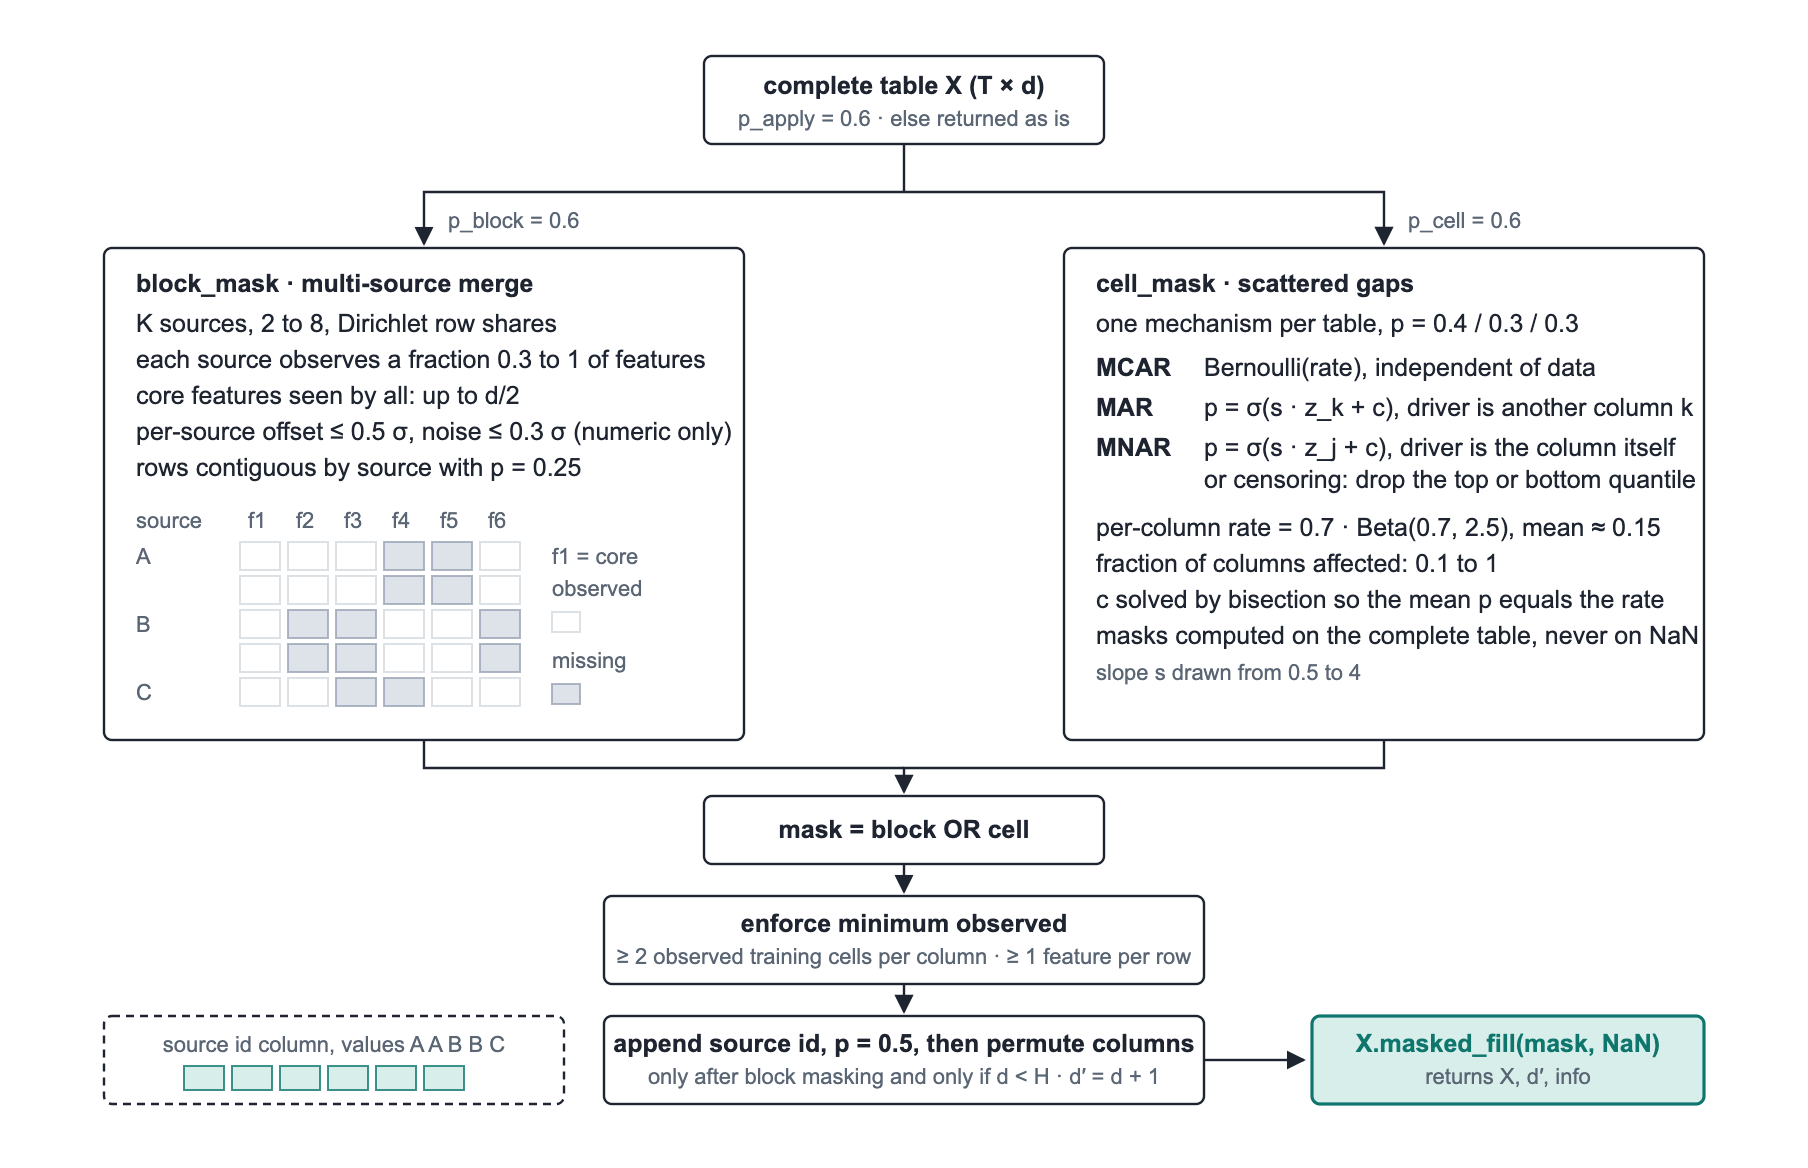
\includegraphics[width=0.95\linewidth]{figures/mechanism.png}
\caption{How a complete synthetic table becomes an incomplete one: block masking by
source, cell-wise masking, their union, the safety rules and the optional source-id
column.}
\label{fig:mech}
\end{figure}

\paragraph{Recipe.} Training continues from the released TabICLv2 classifier and
regressor. Stage 4 runs 10\,000 steps at batch 32 with sequences of 400 to 8\,192 rows
and up to 100 features, Muon optimiser, cosine schedule, learning rate $5\times
10^{-5}$, block reconstruction with weight 0.1, offset consistency with weight 0.1 on a
quarter of the micro-batches. Stage 4b continues for another 10\,000 steps at
$3\times10^{-5}$ on the stronger source effects given above, because the stage-4
model's consistency loss had fallen to 0.005, showing it was invariant to the shifts
it saw but not yet to the larger ones of the evaluation. Each stage takes about 9.5
hours per task on one NVIDIA RTX~5090 in bfloat16 (2.7--3.3 s per step); the second
view of the consistency loss adds about 15\,\%. The classifier's task loss fell from
0.60 to 0.57 while the reconstruction loss fell from 0.21 to 0.19 and the consistency
loss stayed near 0.005; the regressor's pinball loss stayed near 0.08. The classifier
has 27.7\,M parameters and the regressor 28.7\,M, against 27.6\,M and 28.5\,M for
TabICLv2: the additions cost 0.1--0.2\,M.

\paragraph{Engineering notes.} Two details mattered in practice. Under distributed data
parallel, an out-of-memory micro-batch that was skipped while gradient synchronisation
was armed left the reducer waiting for a backward pass that never came; gradients are
now averaged by hand after the micro-batch loop, which makes skipped micro-batches and
parameters unused in a micro-batch harmless. And the zero-initialised parameters must
still take part in every backward pass, so the all-false mask is kept in training mode
and an empty reconstruction loss is written as $0\cdot\sum\theta_{\text{head}}$.

\section{Experiments}
\label{sec:experiments}

\paragraph{Protocol.} Twenty public datasets (13 classification, 7 regression; from
scikit-learn and OpenML, subsampled to at most 3\,000 rows), block and block\_shift
missingness at rates 0.3 and 0.5, five seeds, both splits of Section~\ref{sec:headroom}:
about 400 conditions per split. Models: the released TabICLv2 with mean imputation
(``TabICLv2''), TabICL-M, TabPFN~2.5 and TabPFN-3 at their default settings and public
checkpoints, and CatBoost. All in-context learners use eight ensemble members. We report
the mean rank over the five models (1 = best), paired win/loss counts against TabPFN-3
on identical splits and deleted cells, and the number of datasets on which the
per-dataset mean is better. Everything is reproducible from the repository
(\texttt{results/broad}).

\begin{table}[t]
\centering\small
\caption{Mean rank over five models (1 = best) on the 20-dataset benchmark; paired
counts and datasets won are TabICL-M against TabPFN-3.}
\label{tab:main}
\begin{tabular}{llccccc|c}
\toprule
task & split, condition & \textbf{TabICL-M} & TabPFN-3 & TabPFN 2.5 & TabICLv2 & CatBoost & vs TabPFN-3\\
\midrule
\multicolumn{8}{l}{\emph{Classification, 13 datasets}}\\
& held-out source, with offset & \textbf{2.35} & 2.41 & 2.48 & 3.08 & 4.68 & 61/69, 9 of 13\\
& held-out source, all & 2.36 & 2.36 & 2.58 & 3.01 & 4.69 & 123/133, 9 of 13\\
& held-out source, no offset & 2.37 & \textbf{2.31} & 2.68 & 2.94 & 4.70 & 62/64, 7 of 13\\
& random split & \textbf{2.35} & 2.45 & 2.69 & 2.77 & 4.74 & 131/120, 8 of 13\\
\midrule
\multicolumn{8}{l}{\emph{Regression, 7 datasets}}\\
& held-out source, with offset & \textbf{1.97} & 2.53 & 2.63 & 3.44 & 4.43 & \textbf{44/26, 5 of 7}\\
& held-out source, all & 2.24 & \textbf{2.14} & 2.61 & 3.41 & 4.61 & 67/73, 3 of 7\\
& held-out source, no offset & 2.50 & \textbf{1.74} & 2.59 & 3.37 & 4.80 & 23/47, 2 of 7\\
& random split & 2.79 & \textbf{1.79} & 2.75 & 3.00 & 4.67 & 42/98, 1 of 7\\
\midrule
\multicolumn{8}{l}{\emph{Both tasks, 20 datasets}}\\
& held-out source, with offset & \textbf{2.22} & 2.45 & 2.53 & 3.21 & 4.59 & \textbf{105/95, 14 of 20}\\
& held-out source, all & 2.32 & \textbf{2.28} & 2.59 & 3.15 & 4.66 & 190/206, 12 of 20\\
& random split & 2.51 & \textbf{2.22} & 2.71 & 2.85 & 4.71 & 173/218, 9 of 20\\
\bottomrule
\end{tabular}
\end{table}

\subsection{Main results}

Table~\ref{tab:main} is the result. When a held-out source carries a measurement
offset, TabICL-M ranks first on both tasks and pooled (2.22 against 2.45 for TabPFN-3
and 2.53 for TabPFN~2.5) and wins 14 of 20 datasets against TabPFN-3; on regression the
margin is clear (44 wins to 26, 2.1\,\% lower RMSE, 5 of 7 datasets). On classification
it is level with TabPFN-3 everywhere: identical rank over all held-out-source
conditions, a touch ahead on random splits and under offset, and the differences are
0.002--0.005 AUC, inside seed noise. On regression without an offset TabPFN-3 leads
clearly (23/47 under a held-out source, 42/98 on random splits). Against every other
model TabICL-M wins every summary on both tasks: 219/177 and 16 of 20 datasets against
TabPFN~2.5, 281/116 and 18 of 20 against the released TabICLv2 under held-out sources.
Against its own base the improvement is largest where it was designed to be: on
regression under a held-out source it lowers RMSE by 8.5\,\% with offset (59 wins, 11
losses, 7 of 7 datasets; diamonds 2935 to 2208, diabetes 69.1 to 65.1) and 6.1\,\%
without, while on complete data the two are within 0.7\,\% (17 wins, 18 losses).
Under a held-out source the regressor is also better calibrated: its 80\,\% interval
covers 0.81 with a width of 1.6 target standard deviations, where TabICLv2 over-covers
at 0.87 with width 2.1.

\begin{figure}[t]
\centering
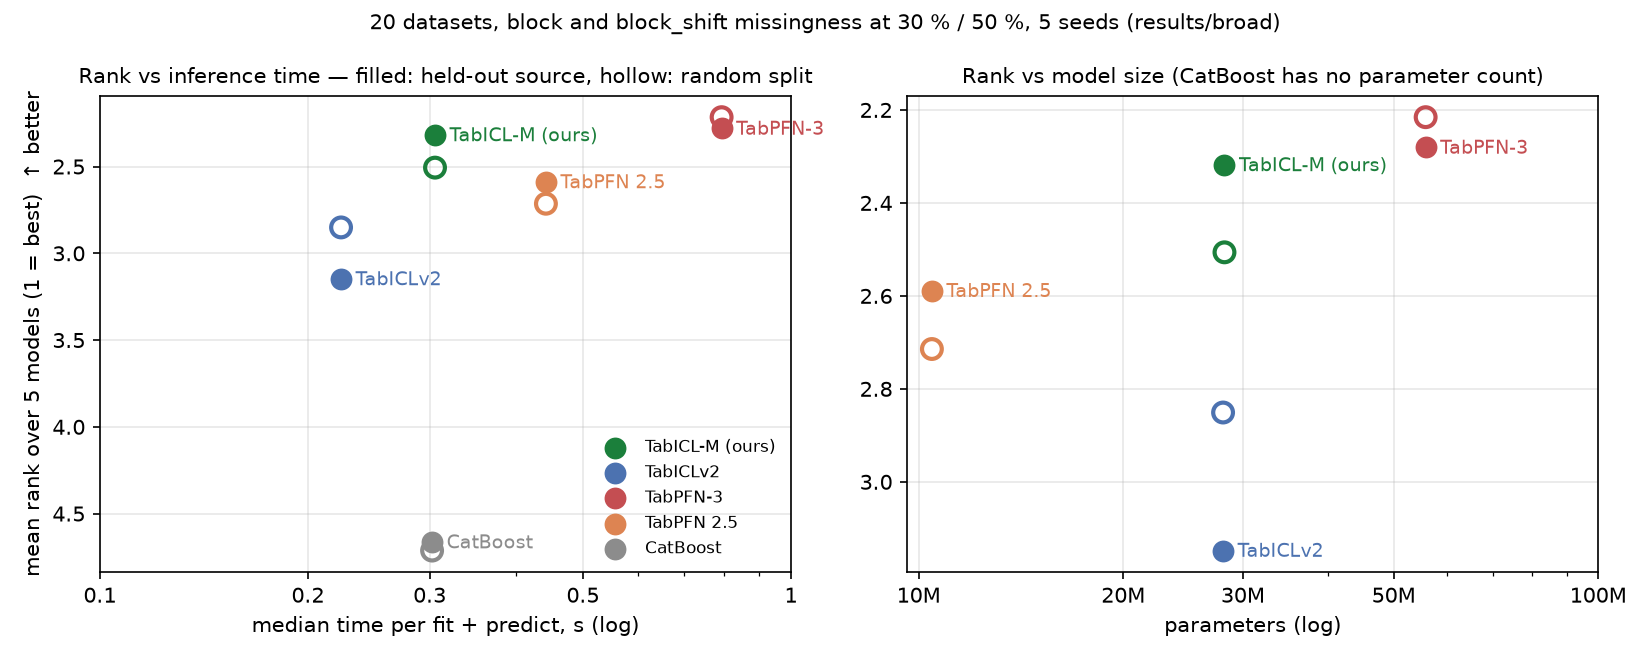
\includegraphics[width=\linewidth]{figures/rank_vs_time_params.png}
\caption{Mean rank on all incomplete conditions of the benchmark against median
inference time (fit plus predict, one RTX~5090, eight ensemble members) and against
parameter count. Filled: held-out source; hollow: random split. TabICL-M matches
TabPFN-3 with half the parameters and a third of the time and improves on TabICLv2,
equal in size and speed, by 0.8 rank points on held-out sources.}
\label{fig:cost}
\end{figure}

\subsection{Cost}

Figure~\ref{fig:cost} places accuracy against cost. TabICL-M (28\,M parameters, 0.3\,s
per fit and predict) matches TabPFN-3 (56\,M, 0.8\,s) in rank and is the most accurate
model per parameter and per second among the foundation models; TabPFN~2.5 is smaller
(10.5\,M) but ranks behind both. Because the additions cost 0.2\,M parameters and one
extra read-out, TabICL-M has the size and speed of TabICLv2 while being 0.8 rank points
better on held-out sources.

\subsection{TabArena-style scoring}

TabArena \citep{erickson2025tabarena} scores methods by Elo from pairwise comparisons per
task, with bootstrap confidence intervals, alongside rank, win rate and improvability. We
apply its evaluator to the same runs, treating each (dataset, mechanism, rate) as a task
and each seed as a repeat, with log loss for classification and RMSE for regression as
the error and Elo anchored to TabICLv2 at 1000 (Figure~\ref{fig:elo},
Table~\ref{tab:elo}). On held-out sources TabICL-M leads TabPFN-3 by 58 Elo (1325
against 1267; win rate 0.80 against 0.73; mean reciprocal rank 0.70 against 0.61) at a
third of its inference time; on random splits TabPFN-3 leads by 38 Elo with confidence
intervals of several hundred points, a tie. CatBoost trails both splits by more than 400
Elo.

\begin{figure}[t]
\centering
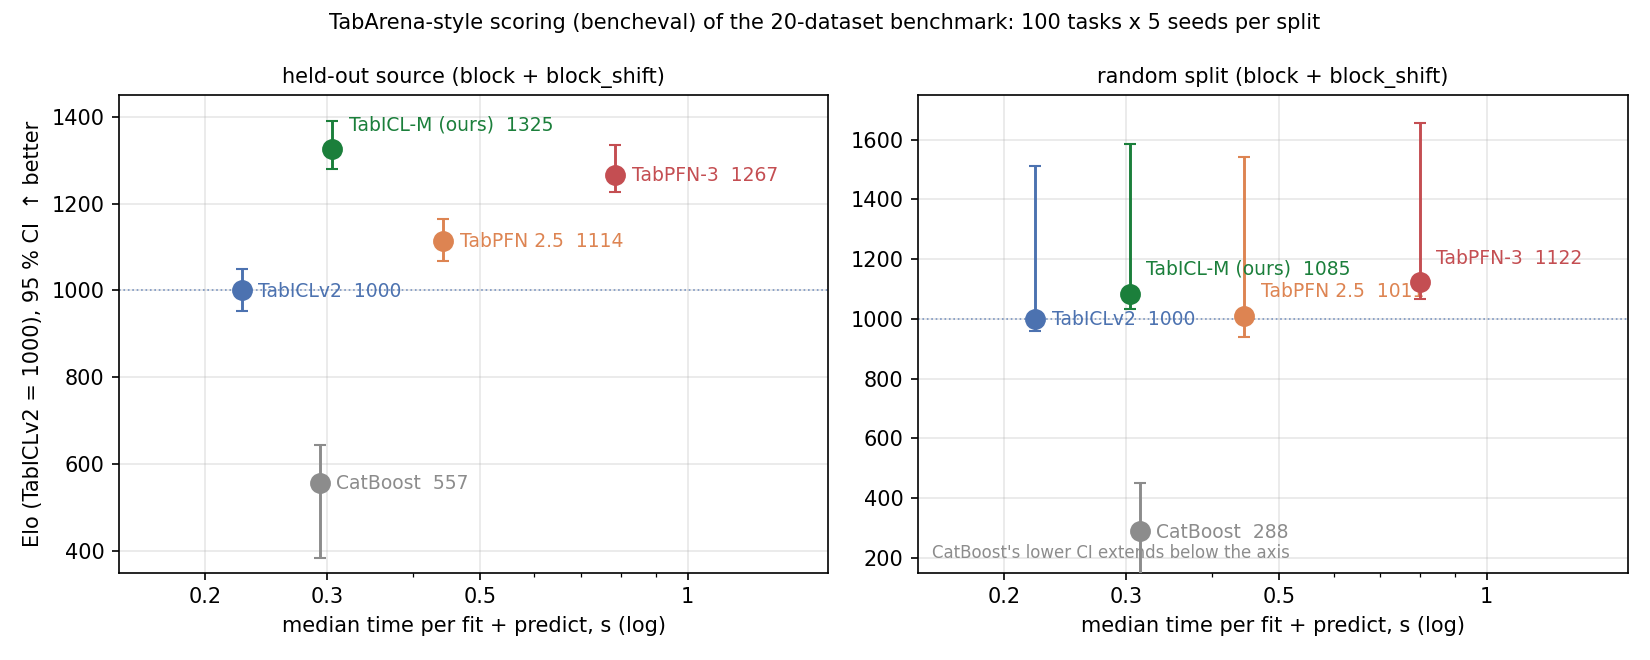
\includegraphics[width=\linewidth]{figures/elo_vs_time.png}
\caption{TabArena-style scoring of the benchmark: Elo with 95\,\% bootstrap confidence
intervals, anchored to TabICLv2 at 1000, against median inference time (fit plus predict,
one RTX~5090). 100 tasks $\times$ 5 seeds per split. CatBoost's lower interval on the random
split extends below the axis.}
\label{fig:elo}
\end{figure}

\begin{table}[t]
\centering\small
\caption{TabArena-style leaderboard of the benchmark (bencheval). Elo anchored to
TabICLv2 = 1000; improvability is the mean relative distance to the best method per task.}
\label{tab:elo}
\begin{tabular}{lcccccc}
\toprule
& \multicolumn{3}{c}{held-out source} & \multicolumn{3}{c}{random split}\\
model & Elo (95\,\% CI) & rank & win rate & Elo (95\,\% CI) & rank & win rate\\
\midrule
TabICL-M (ours) & \textbf{1325} ($+65/-45$) & \textbf{1.79} & \textbf{0.80} & 1085 ($+500/-51$) & 2.34 & 0.67\\
TabPFN-3 & 1267 ($+68/-40$) & 2.07 & 0.73 & \textbf{1122} ($+533/-54$) & \textbf{2.13} & \textbf{0.72}\\
TabPFN 2.5 & 1114 ($+51/-46$) & 2.86 & 0.54 & 1011 ($+533/-70$) & 2.76 & 0.56\\
TabICLv2 & 1000 ($+50/-47$) & 3.42 & 0.40 & 1000 ($+512/-42$) & 2.82 & 0.55\\
CatBoost & 557 ($+87/-175$) & 4.86 & 0.04 & 288 ($+162/-2005$) & 4.95 & 0.01\\
\bottomrule
\end{tabular}
\end{table}

\subsection{Ablation}
\label{sec:ablation}

Each part has a switch. Table~\ref{tab:abl} trains one variant per switch for 3\,000
steps on the source-aware prior and evaluates it on the held-out-source-with-offset
condition; for the classifier the metric is the win rate against mean imputation, for
the regressor the mean RMSE gain over the released regressor.

\begin{table}[t]
\centering\small
\caption{Ablation on held-out sources with offset. Classifier: win rate against mean
imputation (4 datasets). Regressor: mean RMSE gain over the released regressor (7
datasets). One switch off at a time, 3\,000 steps each.}
\label{tab:abl}
\begin{tabular}{lcc}
\toprule
variant & classifier win rate & regressor RMSE gain\\
\midrule
all parts on & 0.73 & $+5.1\,\%$\\
without source-relative values & 0.70 & $+4.9\,\%$\\
without observed-only rows & 0.68 & $+4.8\,\%$\\
without pattern token & 0.65 & $+5.3\,\%$\\
without block reconstruction and consistency & 0.70 & $+5.1\,\%$\\
all parts off (new prior only) & 0.62 & $+4.5\,\%$\\
first checkpoint (old prior, value-level parts) & 0.62 & ---\\
all parts on, full training (10k / 20k steps) & 0.77 & $+8.6\,\%$\\
\bottomrule
\end{tabular}
\end{table}

For the classifier every part helps, the pattern token and the observed-only rows
most, and the new prior alone adds nothing over the first checkpoint: the gain is in
the architecture. For the regressor the picture differs in one respect: the prior
alone already gives $+4.5\,\%$, the parts add about one point at 3\,000 steps, and
training length adds the rest, to $+8.6\,\%$ at 20\,000 steps, the only variant ahead
of TabPFN-3 there. No part hurts either task on complete data (every regression
variant is within $+0.2$ to $+1.0\,\%$ of the released regressor), so the parts are
safe to keep on everywhere.

\subsection{What did not close the regression gap}
\label{sec:negative}

The one place TabPFN-3 leads is regression without a source offset. We probed it
exhaustively, on kin8nm, space\_ga and diamonds where the gap is largest (5--15\,\% on
complete data), and report the results because they locate the cause.
\emph{Test-time levers}: 32 ensemble members, the median instead of the mean, a
target power-transform ensemble and an extra quantile-normalisation member improve our
own ranking slightly and leave the head-to-head unchanged (41 wins, 97 losses on random
splits); TabPFN-3 gains nothing from 32 members either. \emph{Weight soup} of the 10k
and 20k regressors: $+0.08\,\%$. \emph{Continued training} on a prior with half the
tables complete: 85 wins, 90 losses against the 20k model after 3\,500 steps, stopped.
\emph{Test-time fine-tuning} on the context rows recovers a third of the kin8nm gap
(0.0761 to 0.0736 against 0.0721) and half of space\_ga's, then plateaus at 100 epochs;
TabPFN-3 fine-tuned the same way on the same rows gets slightly worse, so its zero-shot
model stays best. \emph{A TabPFN-style histogram head} (1\,000 per-table equal-mass
buckets, log-density loss, output layer from zero, 20\,000 steps) is worse than the
quantile head on every regression dataset on complete data (9 wins, 26 losses, 7\,\%
higher RMSE). \emph{A sample-efficiency curve} shows the kin8nm gap at every training
size, narrowing from 13\,\% at 300 rows to 5\,\% at 2\,100, so it is not a limitation of
in-context learning from little data; and TabPFN~2.5, with 10\,M parameters, beats us
there too, so it is not capacity. What remains is the quality of the base regressor on
smooth nonlinear functions, inherited from TabICLv2 (whose released regressor ranks
6.4 against TabPFN-3's 4.0 on these datasets under a held-out source) and not touched by
missingness training, adaptation on the context, or the output distribution.

\section{Discussion}
\label{sec:discussion}

\paragraph{Where the method pays and why.} The gain of TabICL-M is confined to the
regime it was built for, and that is the honest reading of Table~\ref{tab:main}. Under a
random split every source is in the context and there is nothing for a source-aware
mechanism to fix; under a held-out source without offset the missing block is a loss of
information that no representation can undo; only under a held-out source with an
offset is there a nuisance to remove, and there TabICL-M removes more of it than any
other model. The ablation supports the mechanism: the pattern token, which carries the
source identity, and the observed-only rows, which let a row from a new feature
combination be represented at all, are the two parts that matter most for
classification, and the first-generation checkpoint, which could see \emph{that} a cell
was missing but not \emph{which source} a row came from, gained nothing.

\paragraph{Cost of a foundation-model comparison.} The comparison against TabPFN-3
would have been misleading without the paired design, the by-task split and the
negative results. Pooled over both tasks TabICL-M is a close second to TabPFN-3 (2.32
against 2.28); split by task it is level on classification and the whole deficit is
regression without offset; probed further, that deficit is the base regressor's. Each
of these statements is weaker than the one before, and each is the one that survives.

\paragraph{Limitations.} All source structure in the benchmark is synthetic, imposed on
complete public tables; the leave-one-laboratory-out test on the compaction database
that motivated the work has not been run. Five seeds give paired win rates of 52--57\,\%
under offset against TabPFN-3, a rank difference rather than a significant margin per
dataset. TabArena and BeyondArena, whose datasets are complete, cannot show the effect
we target; our TabArena-Lite and BeyondArena grouped-split runs are in progress and
will be reported in the repository, with the expectation of a TabICLv2-level placement
on TabArena. Finally, one RTX~5090 and 20\,000 continuation steps are a small budget
against the pre-training of TabPFN-3, and we do not claim to have exhausted what a
larger one would give the base regressor.

\section{Conclusion}

Merged engineering databases are incomplete in a structured way: each source measured
its own columns on its own scale. We showed that this is the one regime in which current
tabular foundation models leave a recoverable gap, and that reading a row's missingness
pattern as its provenance, through a source-relative value encoding, observed-only row
attention and a pattern token trained on a source-structured prior, recovers it.
TabICL-M is the best model of any kind when a new source arrives with its own
calibration, level with TabPFN-3 on classification, and behind it only on plain
regression, at half the parameters and a third of the inference time. The parts are
zero-initialised, so nothing that TabICLv2 does on complete data is lost. The weights,
the code, the benchmark and every negative result are public.

\paragraph{Acknowledgements.} TabICL-M is a fork of TabICL by Jingang Qu, David
Holzm\"uller, Ga\"el Varoquaux and Marine Le Morvan, whose released weights, prior and
training code it builds on.

\begin{thebibliography}{99}
\small

\bibitem[Caruso et al.(2024)]{caruso2024naim}
C. M. Caruso, P. Soda, V. Guarrasi.
Not another imputation method: A transformer-based model for missing values in tabular datasets.
\emph{arXiv:2407.11540}, 2024; \emph{AI Open}, 2026.

\bibitem[Du et al.(2024)]{du2024remasker}
T. Du, L. Melis, T. Wang.
ReMasker: Imputing tabular data with masked autoencoding.
\emph{ICLR}, 2024. arXiv:2309.13793.

\bibitem[Erickson et al.(2025)]{erickson2025tabarena}
N. Erickson, L. Purucker, A. Tschalzev, D. Holzm\"uller, P. M. Desai, D. Salinas, F. Hutter.
TabArena: A living benchmark for machine learning on tabular data.
\emph{NeurIPS}, 2025. arXiv:2506.16791.

\bibitem[Hollmann et al.(2023)]{hollmann2023tabpfn}
N. Hollmann, S. M\"uller, K. Eggensperger, F. Hutter.
TabPFN: A transformer that solves small tabular classification problems in a second.
\emph{ICLR}, 2023.

\bibitem[Hollmann et al.(2025)]{hollmann2025tabpfnv2}
N. Hollmann, S. M\"uller, L. Purucker, A. Krishnakumar, M. K\"orfer, S. B. Hoo, R. T. Schirrmeister, F. Hutter.
Accurate predictions on small data with a tabular foundation model.
\emph{Nature}, 637:319--326, 2025.

\bibitem[Lee et al.(2019)]{lee2019set}
J. Lee, Y. Lee, J. Kim, A. Kosiorek, S. Choi, Y. W. Teh.
Set Transformer: A framework for attention-based permutation-invariant neural networks.
\emph{ICML}, 2019.

\bibitem[Li et al.(2016)]{li2016adabn}
Y. Li, N. Wang, J. Shi, J. Liu, X. Hou.
Revisiting batch normalization for practical domain adaptation.
\emph{arXiv:1603.04779}, 2016.

\bibitem[Prior Labs(2025--2026)]{priorlabs2026tabpfn3}
Prior Labs.
TabPFN-2.5 and TabPFN-3: model releases and technical reports.
\url{https://huggingface.co/Prior-Labs}, 2025--2026.

\bibitem[Purucker et al.(2026)]{beyondarena2026}
L. Purucker, A. Tschalzev, N. Erickson, G. Blayer, D. Holzm\"uller, A. Arazi, A. Pfefferle, M. Tajjar, G. Varoquaux, F. Hutter.
Beyond IID: How general are tabular foundation models, really?
\emph{arXiv:2606.30410}, 2026.

\bibitem[Qu et al.(2025)]{qu2025tabicl}
J. Qu, D. Holzm\"uller, G. Varoquaux, M. Le Morvan.
TabICL: A tabular foundation model for in-context learning on large data.
\emph{ICML}, 2025. arXiv:2502.05564.

\bibitem[Qu et al.(2026)]{qu2026tabiclv2}
J. Qu, D. Holzm\"uller, G. Varoquaux, M. Le Morvan.
TabICLv2: A better, faster, scalable, and open tabular foundation model.
\emph{arXiv:2602.11139}, 2026.

\bibitem[Rubin(1976)]{rubin1976inference}
D. B. Rubin.
Inference and missing data.
\emph{Biometrika}, 63(3):581--592, 1976.

\bibitem[van Buuren and Groothuis-Oudshoorn(2011)]{vanbuuren2011mice}
S. van Buuren, K. Groothuis-Oudshoorn.
mice: Multivariate imputation by chained equations in R.
\emph{Journal of Statistical Software}, 45(3):1--67, 2011.

\bibitem[Yoon et al.(2020)]{yoon2020vime}
J. Yoon, Y. Zhang, J. Jordon, M. van der Schaar.
VIME: Extending the success of self- and semi-supervised learning to tabular domain.
\emph{NeurIPS}, 2020.

\end{thebibliography}

\end{document}
